\documentclass{beamer}
\usepackage[spanish]{babel}
\usepackage[utf8]{inputenc}
\usepackage{multicol}
\usepackage{soul}

\usepackage[
    type={CC},
    modifier={by-sa},
    version={3.0},
]{doclicense}

\usetheme{Warsaw}
\usecolortheme{crane}
\useoutertheme{shadow}
\useinnertheme{rectangles}

\setbeamertemplate{navigation symbols}{}

\title[XHTML y CSS]{Taller de XHTML y CSS3}
\subtitle{Nivel Básico - Parte I}
\author[Julián Fernández, Rubén Martín]{
	\textbf{Julian Fernández Ortiz }
	\\
	\medskip
	\scriptsize{
	Vicepresidente de IEEE Student Branch of Granada\\
	Grado en Ingeniería Electrónica Industrial
	}	
	\\	
	\texttt{julian.fernandez.es@ieee.org}
	\\ \ \\
	\small{\textbf{Rubén Martín Moreno}}
	\\
	\medskip
	\scriptsize{
	Tesorero de IEEE Student Branch of Granada\\
	Grado en Estadística
	}
	\\
	\texttt{ruben.martinmoreno.es@ieee.org}
}
\date{}

\begin{document}
\frame{\titlepage}

\begin{frame}
\frametitle{Licencia}
\doclicenseThis
Fuente: Curso desarrollado por IEEE Student Branch of Granada
\end{frame}

\begin{frame}
  \frametitle{Índice}
  \tableofcontents
\end{frame}

\section{CONCEPTOS GENERALES}
	\subsection{Estructura de un Sitio Web}
\begin{frame}
  \begin{columns}[c]
    \column{0.4\textwidth}
	\begin{block}{Estructura de Árbol}
	Existe una página principal desde la que puedes llegar a otras páginas de la web
	\end{block}

    \column{0.6\textwidth}
	\begin{center}
	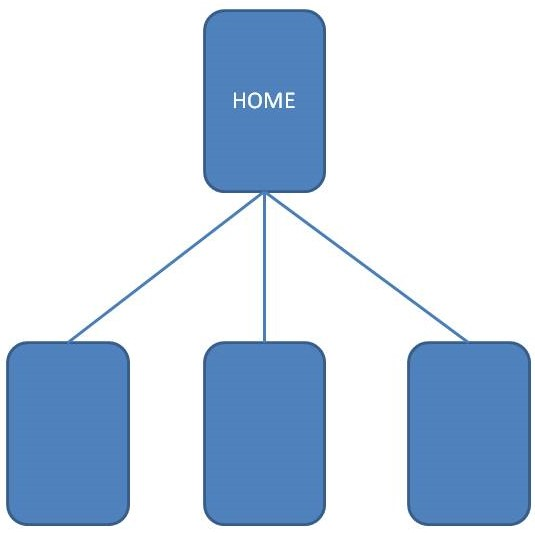
\includegraphics[scale=.3]{images/EstructuraArbol.JPG} 
	\end{center}
  \end{columns}
\end{frame}

\begin{frame}
  \begin{columns}[c]
    \column{0.4\textwidth}
	\begin{block}{Estructura en Listas}
	Las páginas están enlazadas con sus contiguas
	\end{block}

    \column{0.6\textwidth}
	\begin{center}
	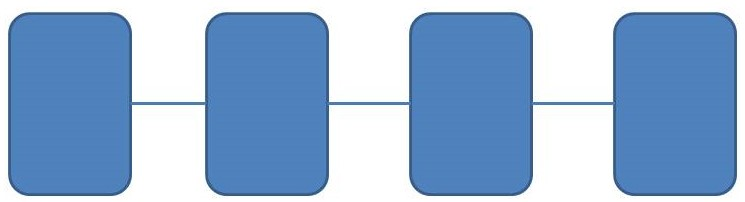
\includegraphics[scale=.3]{images/EstructuraListas.JPG} 
	\end{center}
  \end{columns}
\end{frame}

\begin{frame}
  \begin{columns}[c]
    \column{0.4\textwidth}
	\begin{block}{Estructura Mixta}
	Aprovecha las dos anteriores
	\end{block}

    \column{0.6\textwidth}
	\begin{center}
	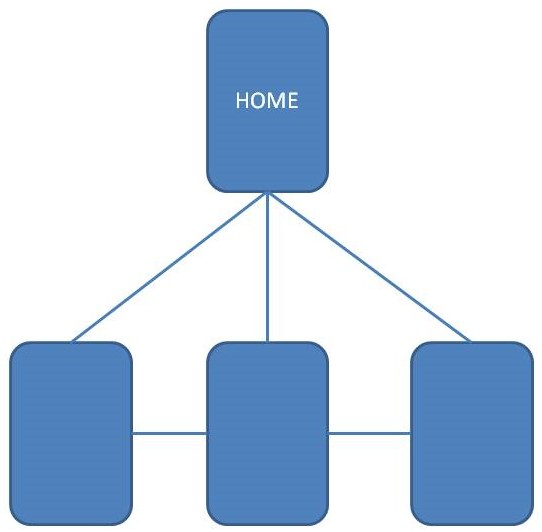
\includegraphics[scale=.3]{images/EstructuraMixta.JPG} 
	\end{center}
  \end{columns}
\end{frame}

\begin{frame}
  \begin{columns}[c]
    \column{0.4\textwidth}
	\begin{block}{Estructura en Red}
	Páginas totalmente interconectadas
	\end{block}

    \column{0.6\textwidth}
	\begin{center}
	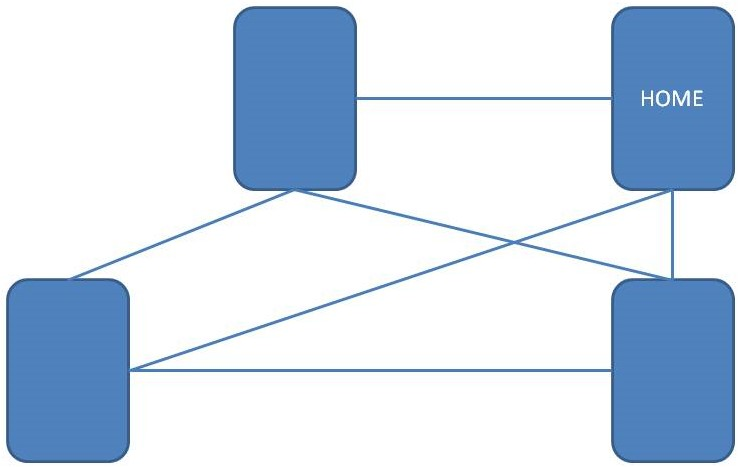
\includegraphics[scale=.3]{images/EstructuraRed.JPG} 
	\end{center}
  \end{columns}
\end{frame}

	\subsection{Los Estándares Web - W3C}
\begin{frame}
\begin{itemize}
\item Se exige que se usen los elementos
	\begin{itemize}
	\item DOCTYPE
	\item HEAD
	\item BODY 
	\item HTML
	\end{itemize}
\item Se exige que se cierren todas las etiquetas
\item Se exige el uso de comillas en torno a valores de atributos
\item Todos los elementos deben estar en minúscula
\item Todos los valores han de indicarse de forma explícita
\end{itemize}
\end{frame}

\begin{frame}[fragile]
\frametitle{W3C}
	\begin{center}
	\verb|https://validator.w3.org/#validate_{}by_{}input|
	\end{center}
\end{frame}

\begin{frame}
\frametitle{W3C}
 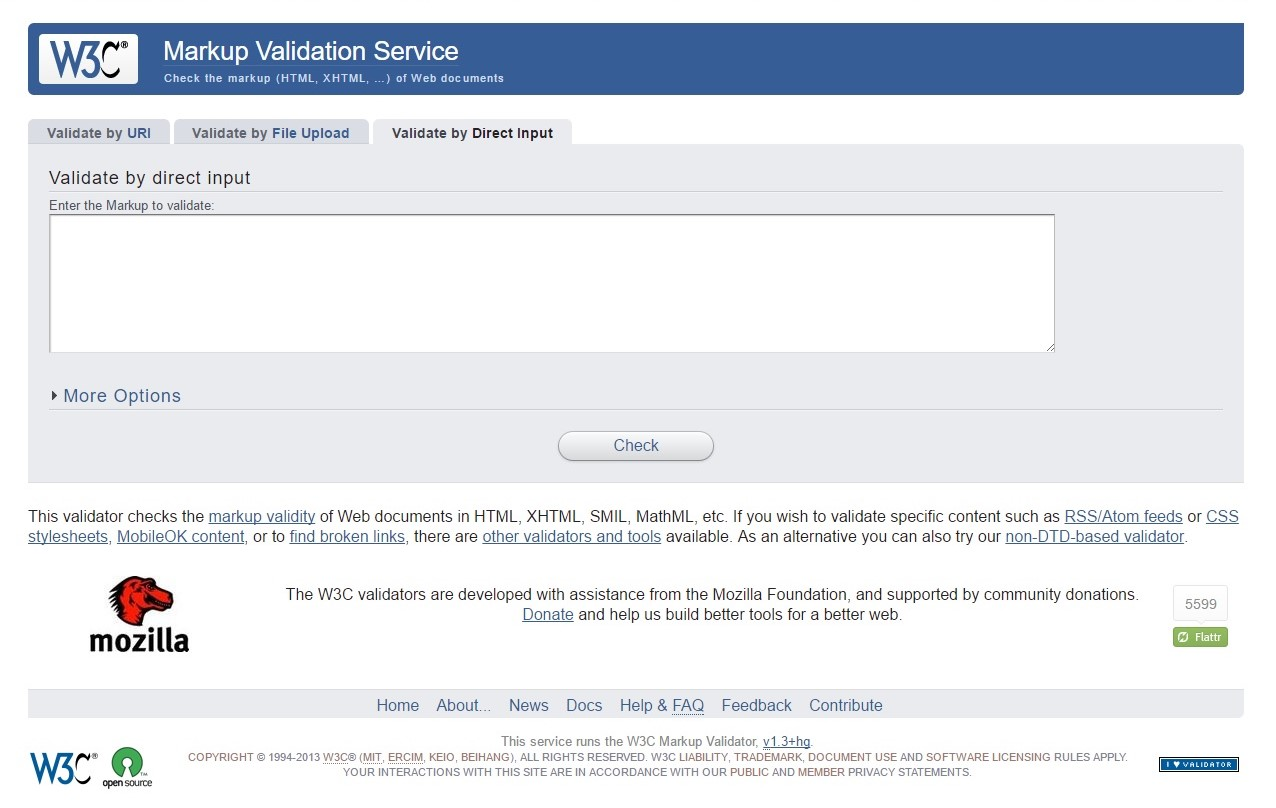
\includegraphics[scale=.32]{images/W3Cvalidator.jpg}
\end{frame}

\section{XHTML}
	\subsection{Estructura de la Página}
\begin{frame}[fragile] %Definición del documento
\frametitle{Definición del Documento}
	\begin{block}{Declaración DOCTYPE}
	\scriptsize{\verb|<!DOCTYPE html PUBLIC "-//W3C//DTD XHTML 1.0 Strict//EN"|}
	\scriptsize{\verb|"http://www.w3.org/TR/xhtml1/DTD/xhtml1-strict.dtd">|}
	\end{block}
	
	\begin{block}{Etiqueta HTML}
	\scriptsize{\verb|<html xmlns="http://www.w3.org/1999/xhtml">|}\\
	\scriptsize{\verb|   ...|}\\
	\scriptsize{\verb|</html>|}
	\end{block}
\end{frame}

\begin{frame}[fragile] %Cabecera
\frametitle{Cabecera}
	\begin{columns}[c]
	\column{0.55\textwidth}
	Incluye:
	\begin{itemize}
	\item Título de la página
	\item Información importante para los motores de búsqueda (Etiquetas)
	\item Ubicación
	\item Hojas de estilos (CSS)
	\item Scripts
	\end{itemize}
	\column{0.45\textwidth}
	\scriptsize{
		\begin{verbatim}
		<head>
		   <title>CURSO XHTML Y CSS</title>
		</head>
		\end{verbatim}
	}
	\begin{alertblock}{IMPORTANTE}
	La declaración de un título para la página es OBLIGATORIA
	\end{alertblock}
	\end{columns}
\end{frame}

\begin{frame}[fragile] %Cabecera - Metadatos
\frametitle{Cabecera}
	\begin{block}{METADATOS más usuales}
	\scriptsize{\verb|<meta charset="UTF-8">|}
	\scriptsize{\verb|<meta name="description" content="CURSO XHTML Y CSS">|}
	\scriptsize{\verb|<meta name="keywords" content="HTML,CSS,XML,XHTML">|}
	\scriptsize{\verb|<meta name="author" content="Julián Fernández; Rubén Martín">|}
	\end{block}
\end{frame}

\begin{frame}[fragile] %Cabecera - Plantilla
\frametitle{Cabecera}
	\scriptsize{
	\begin{verbatim}
	<head>
	
	   <title>CURSO XHTML Y CSS</title>
	   
	   <meta http-equiv="content-type" content="text/html; charset=utf-8"/>
	   <meta http-equiv="Content-Style-Type" content="text/css" />
	   <meta http-equiv="Language" content="Español" />

	   <link href="style.css" rel="stylesheet" type="text/css" />

	   <script><!--SCRIPT--></script>

	</head>
	\end{verbatim}
	}
\end{frame}

\begin{frame}[fragile] %Cuerpo
\frametitle{Cuerpo}
	\begin{columns}[c]
	\column{0.5\textwidth}
	\begin{block}{Contenido de la web}
	Se incluye el texto, imágenes y vídeos que queremos que se muestren en la web
	\end{block}
	
	\column{0.5\textwidth}
	\scriptsize{
	\begin{verbatim}
	<body>
	
	   <!--Contenido de tu Página-->
	   
	</body>
	\end{verbatim}
	}
	\end{columns}
\end{frame}

\begin{frame}[fragile] %Plantilla WEB
\frametitle{En Resumen...}
	\scriptsize{
	\begin{verbatim}
	<!DOCTYPE html PUBLIC "-//W3C//DTD XHTML 1.0 Strict//EN"
	"http://www.w3.org/TR/xhtml1/DTD/xhtml1-strict.dtd">
	<html xmlns="http://www.w3.org/1999/xhtml">
	\end{verbatim}
	\begin{verbatim}
	<head>
	   <title><!--Título en la Pestaña de Búsqueda--></title>
	   <meta http-equiv="content-type" content="text/html; charset=utf-8"/>
	   <meta http-equiv="Content-Style-Type" content="text/css" />
	   <meta http-equiv="Language" content="Español" />

	   <link href="../style/style.css" rel="stylesheet" type="text/css" />
	
	   <!--SCRIPTS-->
	</head>
	\end{verbatim}
	\begin{verbatim}
	<body>
	   <!--Contenido de tu Página-->
	</body>
	\end{verbatim}
	\begin{verbatim}
	</html>	
	\end{verbatim}	
	}
\end{frame}

	\subsection{Etiquetas}
\begin{frame}
	\begin{block}{Tipos de etiquetas más utilizadas (e imprescindibles)}
		\begin{itemize}
		\item Encabezados
		\item Párrafo
		\item Tipología de letra
		\item Script
		\item Código
		\end{itemize}
	\end{block}
\end{frame}

\begin{frame}[fragile]
\frametitle{Encabezados}
	\begin{columns}[c]
	\column{0.1\textwidth}
	\column{0.4\textwidth}
	Son jerárquicos entre sí
	\begin{verbatim}
	<h1>...</h1>
	<h2>...</h2>
	<h3>...</h3>
	<h4>...</h4>
	<h5>...</h5>
	<h6>...</h6>
	\end{verbatim}
	\column{0.45\textwidth}
	\begin{exampleblock}{RECUERDA}
	Cuanto más pequeño es el número más grande la letra
	\end{exampleblock}
	\column{0.05\textwidth}
	\end{columns}
\end{frame}

\begin{frame}[fragile]
\frametitle{Párrafos}
	\begin{columns}[c]
	\column{0.1\textwidth}
	\column{0.4\textwidth}
	Todo el texto debe ir encerrado en párrafos
	\newline
	
	\verb|<p>...</p>|
	\column{0.45\textwidth}
	\begin{exampleblock}{RECUERDA}
	Es bueno separar cada párrafo de manera independiente para que sea más fácil el uso de \textit{identificadores}
	\end{exampleblock}
	\column{0.05\textwidth}
	\end{columns}
\end{frame}

\begin{frame}[fragile]
\frametitle{Párrafos}
	\begin{columns}[c]
	\column{0.5\textwidth}
	\begin{itemize}
	\item \verb|<abbr>...</abbr>|
	\item \verb|<b>...</b>|
	\item \verb|<i>...</i>|
	\item \verb|<em>...</em>|
	\item \verb|<u>...</u>|
	\item \verb|<s>...</s>|
	\item \verb|<sub>...</sub>|
	\item \verb|<sup>...</sup>|
	\end{itemize}
	\column{0.5\textwidth}
	\begin{itemize}
	\item Abreviatura
	\item \textbf{Negrita}
	\item \textit{Cursiva}
	\item \emph{Enfatizado}
	\item \underline{Subrayado}
	\item \textst{Tachado}
	\item Subíndice$_1$
	\item Superíndice$^1$
	\end{itemize}
	\end{columns}
\end{frame}

\begin{frame}[fragile]
\frametitle{Párrafos}
	\begin{block}{Escribir código}
	\verb|                  <code>...</code>|
	\end{block}
\end{frame}
	\subsection{Enlaces}
\begin{frame}[fragile] %Hipervínculos
	\begin{block}{Hipervínculos}
	Los enlaces nos permiten hacer relaciones internas (a secciones) o externas (a otra web o contenido) en nuestra página
	\end{block}
	
	\begin{block}{Estructura Básica}
	\verb|                 <a href="#">...</a>|	
	\end{block}
\end{frame}

\begin{frame}[fragile] %Relaciones internas
\frametitle{Relaciones Internas}
	\begin{columns}[c]
	\column{0.5\textwidth}
	Para crear nuestro punto de llegada deberemos aplicar
	\newline
	
	\verb|<a name="id">...</a>|
	\newline
	
	al texto deseado
	\column{0.5\textwidth}
	Y para el punto de partida aplicamos
	\newline
	
	\verb|<a href="#id">...</a>|
	\end{columns}
\end{frame}

\begin{frame} %Relaciones externas
\frametitle{Relaciones Externas}
	\begin{itemize}
	\item Pueden ser locales o estar alojadas en internet
	\item Enlazan otras webs o archivos
	\end{itemize}
\end{frame}

\begin{frame}[fragile] %Relaciones externas
\frametitle{Relaciones Externas}
	\begin{block}{Internet - WEB}
	\scriptsize{\verb|<a href="http://www.google.com">Google</a>|}
	\end{block}
	\begin{block}{Internet - PDF}
	\scriptsize{\verb|<a href="http://www.ejemplo.com/informe.pdf">Ejemplo [PDF]</a>|}
	\end{block}
	\begin{block}{Local - WORD}
	\scriptsize{\verb|<a href="/informe.doc">Ejemplo [DOC]</a>|}
	\end{block}
	\begin{block}{Local - JPG (En Nueva Pestaña)}
	\scriptsize{\verb|<a href="../imagenes/fondo_escritorio.jpg" target="_blank">|}
	\end{block}
\end{frame}

\begin{frame}[fragile] %Relaciones externas - emails
\frametitle{Relaciones Externas - emails}
	\begin{block}{email en Nueva Pestaña}
	\scriptsize{\verb|<a href="mailto:ieee@ieee.org" target="_blank">Envíanos un email</a>|}
	\end{block}
	\begin{block}{email en Nueva Pestaña + Asunto}
	\scriptsize{\verb|<a href="mailto:ieee@ieee.org?subject=ASUNTO" target="_blank">|
				\verb|   Envíanos un email</a>|}
	\end{block}
	\begin{block}{email en Nueva Pestaña + Texto}
	\scriptsize{\verb|<a href="mailto:ieee@ieee.org?body=TEXTO" target="_blank">|
				\verb|   Envíanos un email</a>|}
	\end{block}	
	\begin{block}{email en Nueva Pestaña + Asunto + Texto}
	\scriptsize{\verb|<a href="mailto:ieee@ieee.org?subject=ASUNTO&body=TEXTO" target="_blank">|
				\verb|   Envíanos un email</a>|}
	\end{block}
\end{frame}

	\subsection{Listas y Tablas}
\begin{frame}
\frametitle{Listas}
	Existen 2 tipos
	\begin{itemize}
	\item Ordenadas
	\item Desordenadas
	\end{itemize}
	\begin{exampleblock}{RECUERDA}
	Las listas se pueden anidar, ya sean del mismo o de distinto tipo
	\end{exampleblock}
\end{frame}

\begin{frame}[fragile]
\frametitle{Listas Ordenadas}
	\begin{columns}[c]
	\column{0.5\textwidth}
	\begin{verbatim}
	<ol>
	    <li>Padre
	    <ol>
	        <li>Hijo1</li>
	        <li>Hijo2</li>
	        <li>Hijo3
	        <ol>
	            <li>Nieto</li>
	        </ol></li>
	    </ol></li>
	</ol>
	\end{verbatim}
	\column{0.5\textwidth}
	\begin{enumerate}
	\item Padre
		\begin{enumerate}
		\item Hijo1
		\item Hijo2
		\item Hijo3
			\begin{enumerate}
			\item Nieto
			\end{enumerate}
		\end{enumerate}
	\end{enumerate}
	\end{columns}
\end{frame}

\begin{frame}[fragile]
\frametitle{Listas Desordenadas}
	\begin{columns}[c]
	\column{0.5\textwidth}
	\begin{verbatim}
	<ul>
	    <li>Padre
	    <ul>
	        <li>Hijo1</li>
	        <li>Hijo2</li>
	        <li>Hijo3
	        <ul>
	            <li>Nieto</li>
	        </ul></li>
	    </ul></li>
	</ul>
	\end{verbatim}
	\column{0.5\textwidth}
	\begin{itemize}
	\item Padre
		\begin{itemize}
		\item Hijo1
		\item Hijo2
		\item Hijo3
			\begin{itemize}
			\item Nieto
			\end{itemize}
		\end{itemize}
	\end{itemize}
	\begin{exampleblock}{RECUERDA}
	Los listas desordenadas son las más utilizadas a la hora de crear menús
	\end{exampleblock}
	\end{columns}
\end{frame}

\begin{frame}[fragile]
\frametitle{Tablas}
	Etiquetas para construir una tabla
	\begin{itemize}
	\item Obligatorias
		\begin{itemize}
		\item \verb|<table>...</table>|
		\item \verb|<tr>...</tr>|
		\item \verb|<td>...</td>|
		\end{itemize}
	\item Opcionales
		\begin{itemize}
		\item \verb|<th>...</th>|
		\end{itemize}
	\end{itemize}
\end{frame}

\begin{frame}[fragile]
\frametitle{Tablas}
	\begin{columns}[c]
	\column{0.5\textwidth}
	\small{
	\begin{verbatim}
	<table>
	  <tr>
	    <td><strong>XHTML</strong></td>
	    <td><strong>CSS</strong></td>
	  </tr>
	  <tr>
	    <td>Contenido</td>
	    <td>Forma</td>
	  </tr>
	  <tr>
	    <td>Texto</td>
	    <td>Formato</td>
	  </tr>
	</table>
	\end{verbatim}
	}
	\column{0.5\textwidth}
	\begin{tabular}{ll}
	\textbf{XHTML} & \textbf{CSS} \\ 
	Contenido & Forma \\ 
	Texto & Formato \\ 
	\end{tabular} 
	\end{columns}
\end{frame}

\begin{frame}[fragile]
\frametitle{Tablas}
	\begin{columns}[c]
	\column{0.5\textwidth}
	\small{
	\begin{verbatim}
	<table>
	  <tr>
	    <th>XHTML</th>
	    <th>CSS</th>
	  </tr>
	  <tr>
	    <td>Contenido</td>
	    <td>Forma</td>
	  </tr>
	  <tr>
	    <td>Texto</td>
	    <td>Formato</td>
	  </tr>
	</table>
	\end{verbatim}
	}
	\column{0.5\textwidth}
	\begin{tabular}{ll}
	\textbf{XHTML} & \textbf{CSS} \\ 
	Contenido & Forma \\ 
	Texto & Formato \\ 
	\end{tabular} 
	\end{columns}
\end{frame}
	\subsection{Multimedia}
\begin{frame}[fragile]
\frametitle{Etiquetas}
	Tipos de etiquetas para insertar contenido externo en la web
	\begin{itemize}
	\item \verb|<img>...</img>|
	\item \verb|<audio>...</audio>|
	\item \verb|<video>...</video>|
	\end{itemize}
\end{frame}

\begin{frame}[fragile]
\frametitle{Imágenes}
	Atributos útiles a la hora de insertar imágenes
	\begin{columns}[c]
	\column{0.5\textwidth}
	\begin{block}{src=``\#"}
	Indica la URL para encontrar la imagen
	\end{block}
	\begin{block}{name=``\#"}
	Nombre de la imagen
	\end{block}
	\begin{block}{alt=``\#"}
	Pequeña descripción de la imagen
	\end{block}
	\column{0.5\textwidth}
	\begin{block}{longdesc=``\#"}
	Indica una URL donde encontrar una descripción más detallada de la imagen
	\end{block}
	\begin{block}{height=``\#"}
	Altura obligada de la imagen
	\end{block}
	\begin{block}{width=``\#"}
	Anchura obligada de la imagen
	\end{block}	
	\end{columns}
\end{frame}	

\begin{frame}[fragile]
\frametitle{Audios}
	Atributos útiles a la hora de insertar audio
	\begin{columns}[c]
	\column{0.5\textwidth}
	\begin{block}{src=``\#"}
	Indica la URL para encontrar el archivo
	\end{block}
	\begin{block}{type=``\#"}
	Indica el tipo de audios: mp3, mpeg, ogg...
	\end{block}
	\begin{block}{autoplay=``\#"}
	Indica si se debe reproducir una vez que el audio se ha cargado (automáticamente)
	\end{block}
	\column{0.5\textwidth}
	\begin{block}{preload=``\#"}
	Especifica si se debe precargar el audio antes de reproducirlo
	\end{block}
	\begin{block}{controls=``\#"}
	Indica los controles que se muestran en pantalla: play, pause...
	\end{block}
	\begin{block}{loop=``\#"}
	Indica si una vez que termine la pista se debe volver a reproducir
	\end{block}	
	\end{columns}
\end{frame}	

\begin{frame}[fragile]
\frametitle{Vídeo}
	Atributos útiles a la hora de insertar vídeos
	\begin{columns}[c]
	\column{0.5\textwidth}
	\begin{block}{src=``\#"}
	Indica la URL para encontrar el archivo
	\end{block}
	\begin{block}{type=``\#"}
	Indica el tipo de vídeo: mp4, mpeg, ogg...
	\end{block}
	\begin{block}{autoplay=``\#"}
	Indica si se debe reproducir el vídeo se ha cargado (automáticamente)
	\end{block}
	\column{0.5\textwidth}
	\begin{block}{preload=``\#"}
	Especifica si se debe precargar el vídeo
	\end{block}
	\begin{block}{controls=``\#"}
	Indica los controles que se muestran en pantalla: play, pause, mute...
	\end{block}
	\begin{block}{loop=``\#"}
	Indica si una vez que termine se debe volver a reproducir
	\end{block}	
	\end{columns}
\end{frame}	

\begin{frame}[fragile]
\frametitle{Vídeo}
	\begin{columns}[c]
	\column{0.5\textwidth}
	\begin{block}{muted=``\#"}
	Indica si el vídeo debe reproducirse sin audio por defecto
	\end{block}
	\begin{block}{poster=``\#" [URL]}
	Indica una imagen que mostrar hasta que el vídeo se reproduzca
	\end{block}
	\column{0.5\textwidth}
	\begin{block}{height=``\#"}
	Altura obligada del vídeo
	\end{block}
	\begin{block}{width=``\#"}
	Anchura obligada del vídeo
	\end{block}
	\end{columns}
\end{frame}	
\end{document}
